\chapter{Data distribution and visualization}
\label{chap:display}

This chapter focuses on user interface and \ac{API} provided by the project. In first section, \ac{API} is described. It serves both user interface and allows integration of external services. The next section covers user interface, graphs and features available to the end user. Python framework Flask requires route declaration so all routes concerning \ac{HTTP} communication are declared in a separate file. File is separated in 3 parts - first part exposes routes to web pages, next part serves \ac{API} functionality while the third part serves data for the graphs.


\section{API interface}

Implemented \ac{API} provides data for both external services and for internal requirements. \ac{URL} for \ac{API} routes is distinguished by \code{/api}. Data served by \ac{API} is in \ac{JSON} format and provides data which application holds. Accessing \code{/api/system} provides the list of all of the nodes with their names, \ac{id}s, the timestamp of latest update and with list of attached sensor \ac{id}s. This allows external services to navigate though the system and query nodes and sensors for values. \code{/api/node} accepts node \ac{id} as a parameter. An example \ac{URL} for accessing node with id 1 would be \code{/api/node?id=1}. This route provides the list of sensors attached to the specific node, timestamp of last update and name. When sensor is accessed using \code{/api/sensor?id=5}, last update, last value, attached node id and position on that node are displayed. If external service wants to access value history for a specific sensor this can be done via route \code{/api/sensor{\_}value} with supplied sensor id as a parameter. If no other parameter is received server will provide last array with 50 latest readings with values accompanied with the timestamp. Filtering can be introduced using start and end timestamps as parameters or readings as number of values that will be provided. An example of data provided by accessing api route with start, end and readings parameters is seen in Listing \ref{lst:api_filter} \\

\begin{lstlisting}[language=json,firstnumber=1,caption={API result for first 5 readings done in a set period of time},label={lst:api_filter}]
  {
    "result": {
      "2017-08-19-19-28-47": 17181, 
      "2017-08-19-19-28-50": 8522, 
      "2017-08-19-19-28-53": 1275, 
      "2017-08-19-19-28-57": 41146, 
      "2017-08-19-19-29-00": 45302
    }
  }
\end{lstlisting}

The next part of the \ac{API} concerns the charts. Most of the charts are implemented using \href{http://www.chartjs.org}{Chart.js} javascript library while \href{https://plot.ly}{plotly} is used for heath map. All of the charts are updated in real time but can also show history so \ac{API} was designed to support these features. The first graph that a user is greeted with is histogram of all sensor values. This graph is for live setup of the sensors and helps users indicate issues with connection or positioning of the sensors. The next graph is sensor graph - for each sensor it shows the history how the values changed through time. The last graph is heath map of the bed which shows the topological preview of the sensor grid. With the increase of weight detected by the sensor, fields become red while with the decrease they become blue. \ac{API} allows user interface to specify the time for which sensor data should be shown. Graph data can be accessed using path \code{/api/chart}.

The last \ac{API} part is 

\section{User interface}

In a case when there is no pressure on the bed, all of the sensors should be at the left of the chart

\begin{figure}[h]
  \begin{center}
    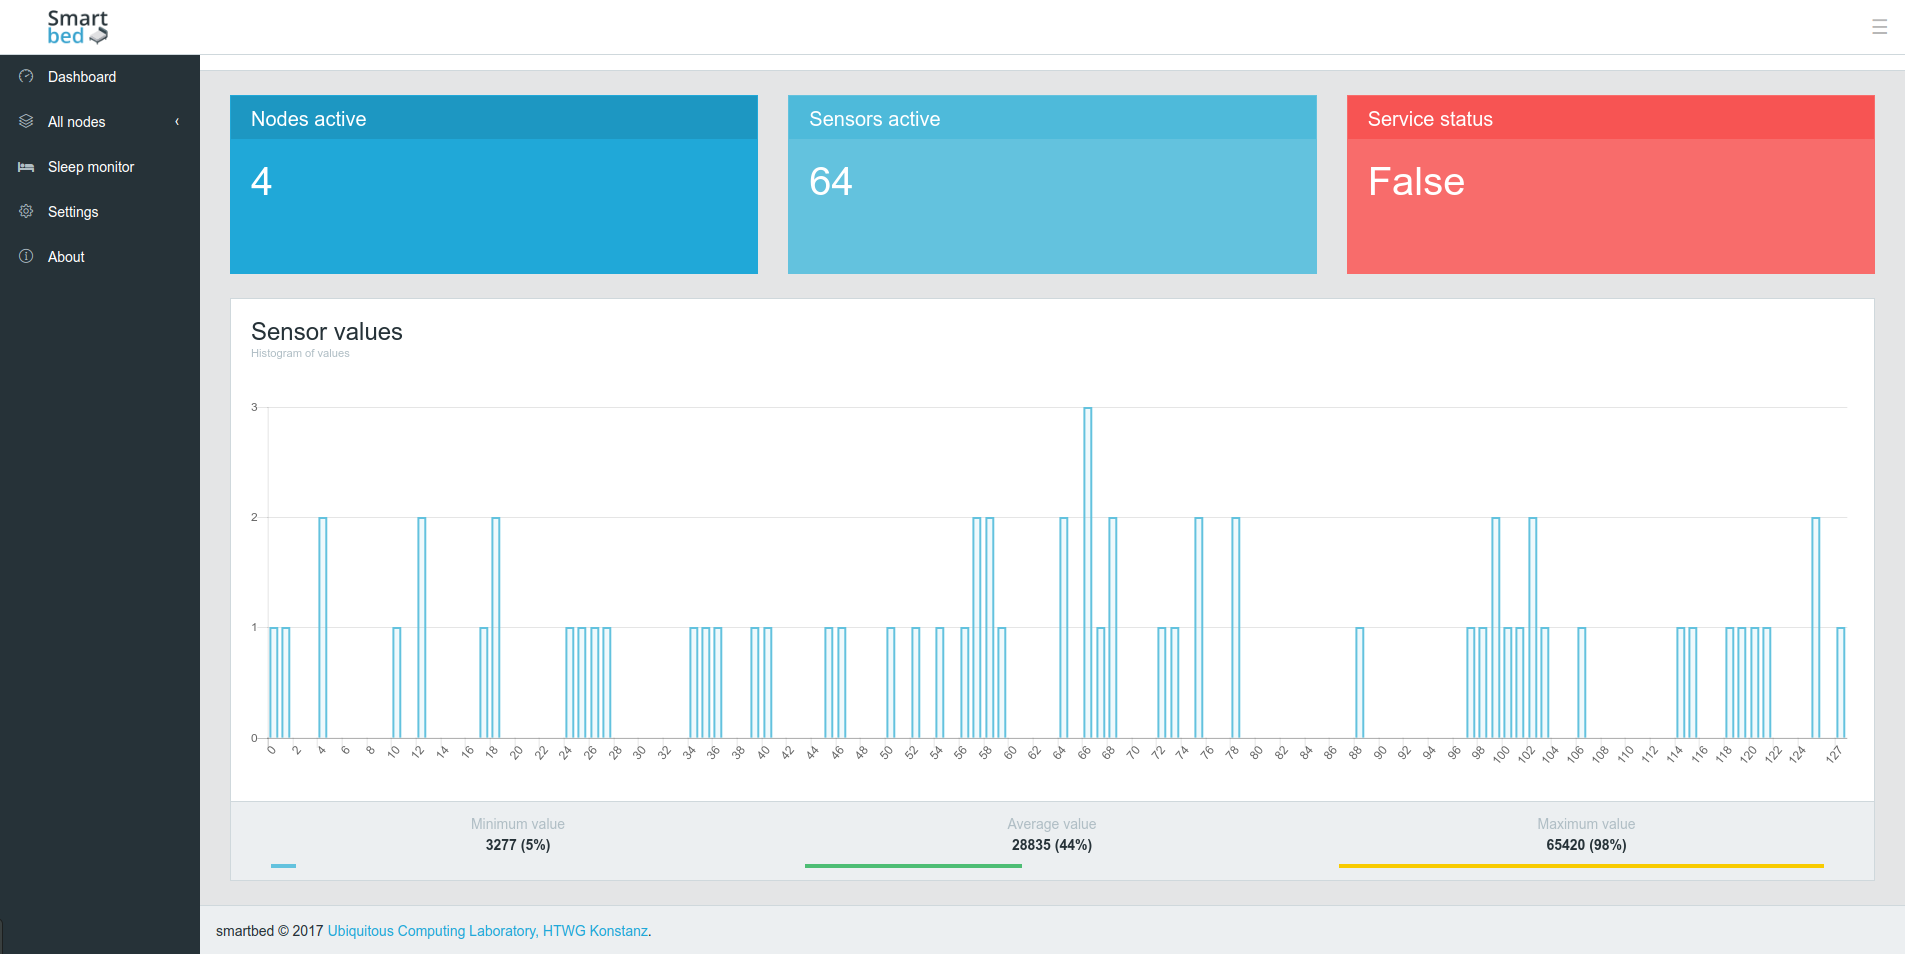
\includegraphics[width=\linewidth]{4-interface_histogram.png}
  \end{center}
  \caption{Flow diagram of data acquisition process.}
  \label{fig:interface_histogram}
\end{figure}

\begin{figure}[h]
  \begin{center}
    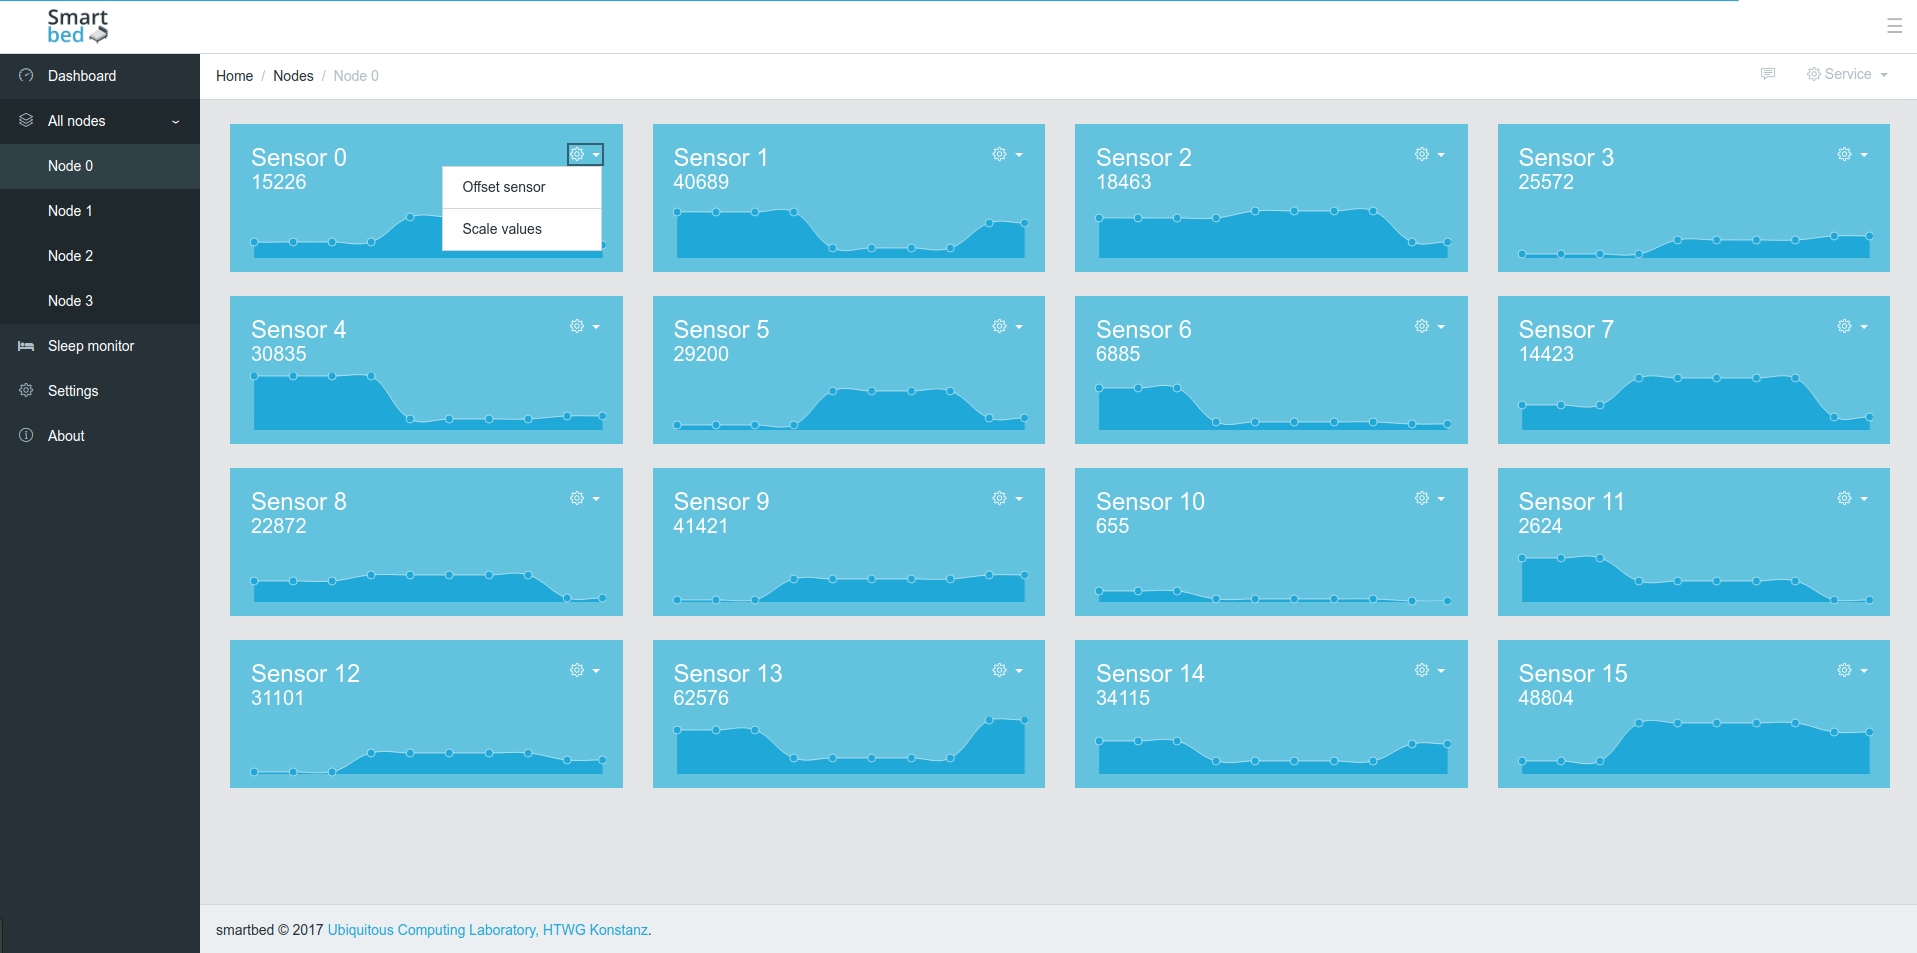
\includegraphics[width=\linewidth]{4-interface_sensors.png}
  \end{center}
  \caption{Flow diagram of data acquisition process.}
  \label{fig:interface_sensors}
\end{figure}

\begin{figure}[h]
  \begin{center}
    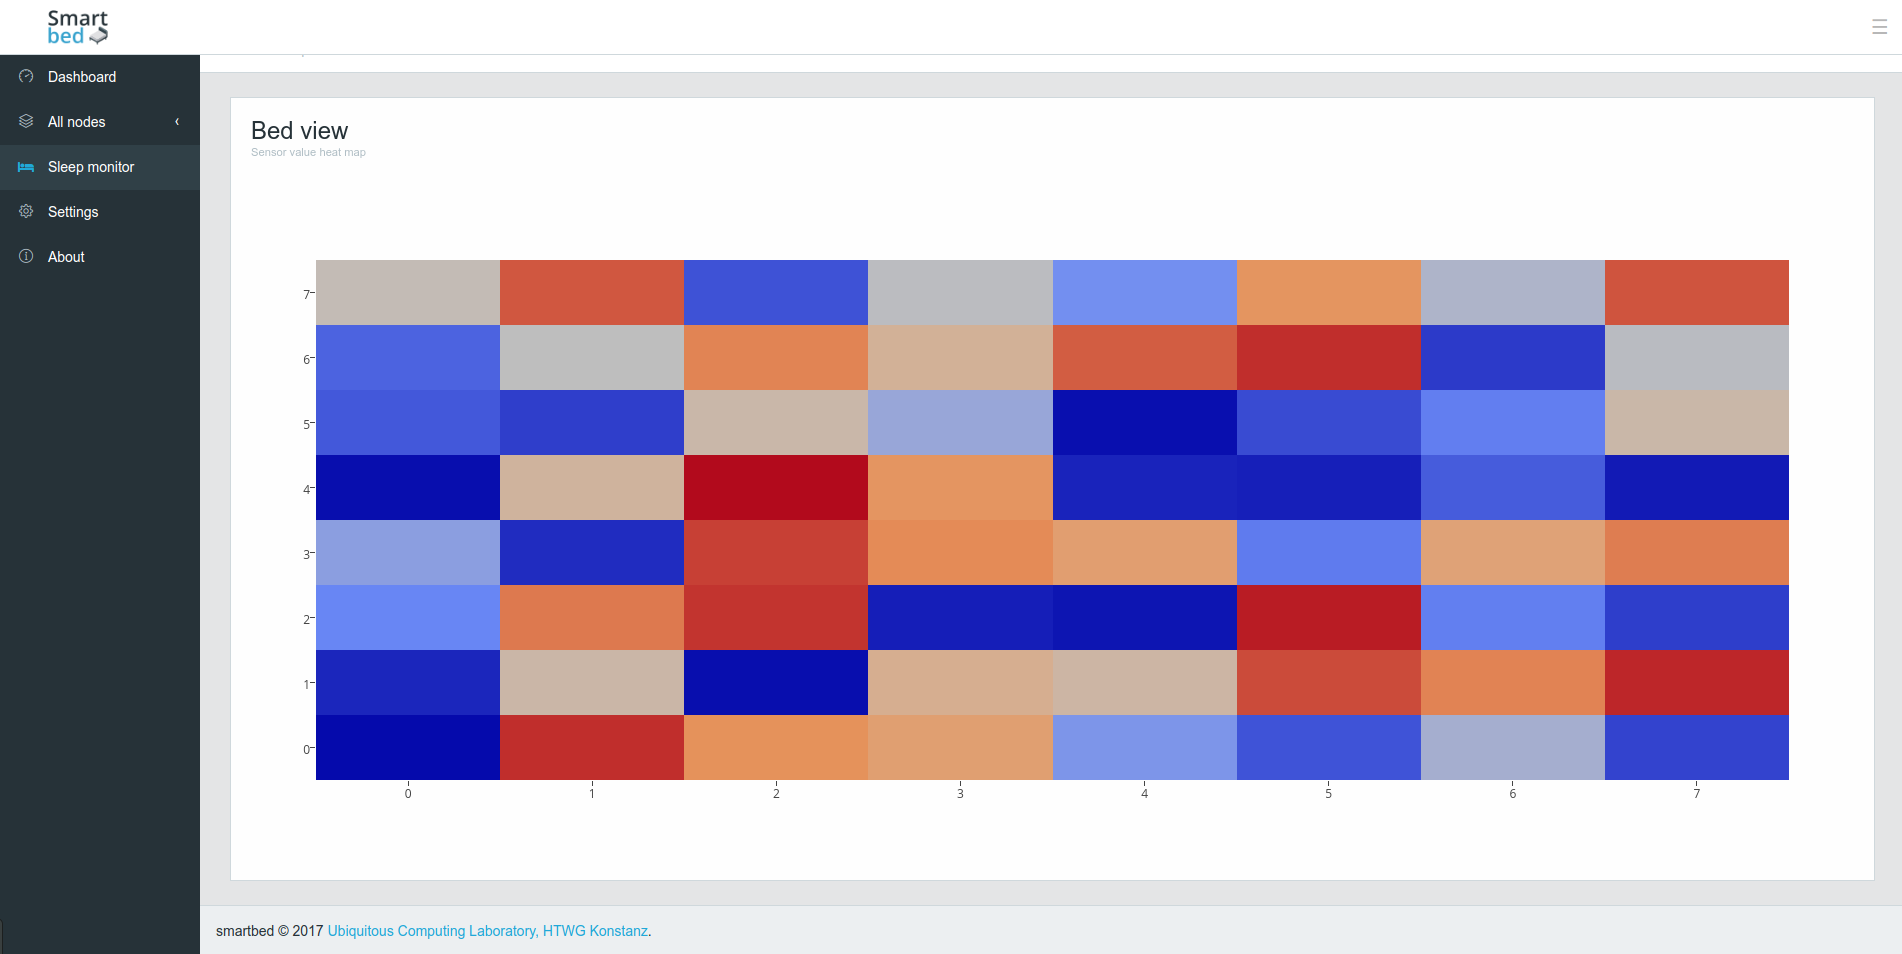
\includegraphics[width=\linewidth]{4-interface_heatmap.png}
  \end{center}
  \caption{Flow diagram of data acquisition process.}
  \label{fig:interface_heatmap}
\end{figure}

\begin{figure}[h]
  \begin{center}
    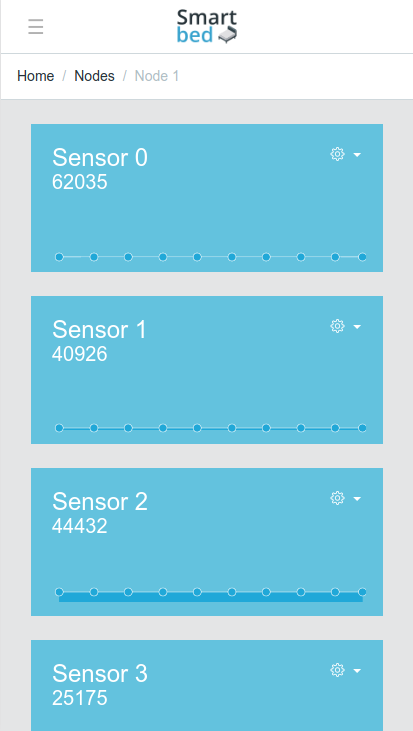
\includegraphics[width=0.4\linewidth]{4-interface_mobile.png}
  \end{center}
  \caption{Flow diagram of data acquisition process.}
  \label{fig:interface_mobile}
\end{figure}